\documentclass[]{article}
\usepackage{pdfpages,amsmath, amssymb, hyperref}
%opening
\title{Formelsammlung Lineare Optimierung \& Stochhastik}
\author{Tobias Reincke}
\date{}
\begin{document}
\setlength{\parindent}{0pt} 

\addtolength{\textwidth}{1.0in}
\addtolength{\textheight}{1.00in}
\addtolength{\evensidemargin}{-0.75in}
\addtolength{\oddsidemargin}{-0.75in}
\addtolength{\topmargin}{-.50in}

\newcommand{\set}[1]{$\{$#1$\}$  }
\includepdf[pages=3, scale=1]{MFETI3.pdf}\includepdf[pages=6, scale=1]{MFETI3.pdf}
\section{Lineare Rekursionsgleichungen}
Derangementzahl: $D_n =(n-1)\cdot(D_{(n-1)}+D_{(n-2)})  \forall n \geq 2\\
D_n=nD_{n-1}+(-1)^n \forall n\geq 1\\ D_0:=1$\\
Charakteristische Gleichung: $p(\lambda)=a_k \lambda^k + a_{k-1} \lambda^{k-1} + a_{k-2} \lambda^{k-2}+ ... + a_0=0$ \\
$c_1 y_n^{ (1) }+c_2 y_n^{(2)}+c_3 y_n^{(3)}+...+c_k y_n^{(k)}$ $\rightarrow$ c ausrechnen 
\subsection{inhomogene}
Störfunktion der Form: $\sum_{k=1}^{n} x_kf_{k}=y$\\
$f_{partikular,n}= c_{n+2}*n^k+\cdots+c_{0}$, $k$ der Grad der Störfunktion (normalerweise 1 oder 2)\\
$\rightarrow$die Partikularformeln mit dem entsprechenden n in der Störfunktion einfügen.\\
\url{https://de.wikipedia.org/wiki/Lineare_Differenzengleichung#Beispiel_2}
$\rightarrow$ nach den Konstanten auflösen.
Anzahl aller surjektiven Abbildungen von A (n) auf B (k) \\ \centering
$\sum_{i=0}^{k} (-1)^i  \binom{n}{k} (k-i)^n$
\\

\section{Körper und Strukturen}
R reflexiv: $\forall$ a aRa \\
R symmetrisch: $\forall$ a,b $\in$ A   aRb $\Rightarrow$ bRa \\
R transitiv: $\forall$ a,b,c $\in$ A aRb $\land$ bRc $\Rightarrow$ aRc \\
R Aquivalenzrelation: $\Leftrightarrow$ R reflexiv, transitiv, symmetrisch \\

Stirling-Zahlen 2. Art (Anzahl der n-elemtigen Mengen in k Klassen): 
$S_{0,0}=1 , S_{n,0}=S_{0,k}=0, n,k \neq 0$
$S_{n,k} = S_{n-1,k-1} + kS_{n-1,k}  $ f\"ur n,k $\geq$ 1 
$S_{n,k}= \frac{1}{k!} \sum_{i=0}^k (-1)^i \binom{k}{i} (k-1)^n$

\subsection{Halb- und Gruppen}
(H,$\odot$) ist Halbgruppe: $\Leftrightarrow$ $\forall a,b,c \in H: a \odot (b \odot c) = (a \odot b) \odot c $ \\
abelsch: $\Leftrightarrow$ $\forall$ a,b $\in$ H: a $\odot$ b = b $\odot$ a \\
Neutrales Element e :  $\Leftrightarrow$ $\forall$ a $\in$ H: a $\odot$ e = e $\odot$ = a \\
(H, $\odot$) Monoid: $\Leftrightarrow$ Halbgruppe mit neutralem Element \\
(H, $\odot$ ) Gruppe: $\Leftrightarrow$ Monoid und alle Elemente invertierbar:\\ $\forall$ a $\in$ H $\exists$ a' $\in$ H : a $\odot$ a' = e  \\
$\forall$ a,b $\in$ H: 
(a $\odot$ b )$^{-1}$ = b$^{-1} \odot $a$^{-1}$\\
a$^i$ = a $\odot$ $\cdot \cdot \cdot$ $\odot$ a $\rightarrow$ Potenzgesetze \\
isomorph: (G1, $\circ_1$) zu (G2, $\circ_2$) seinen Gruppen\\
$\exists$ f$\forall$a,b $\in$ $G_1$ : f(a $\circ_1$ b) = f(a) $\circ_2$ f(b)  

\subsection{Ringe \& Körper}
(R, + , $\cdot$) Ring: $\Leftrightarrow$ 
\begin{itemize}
	 \item (R,+) ist abelsche Gruppe
	 \item (R, $\cdot$) ist Halbgruppe
	 \item $\forall$a,b,c: a $\cdot$ (b + c) = a $\cdot$ b + a $\cdot$ c und (a+b) $\cdot$ c = a $\cdot$ c + b $\cdot$ c 
\end{itemize}
Kommutativ: Halbgruppe ist abelsch
$\sec$
\section{Algorithmen}
\subsection{RSA}
Absender A, Empfänger E \\
E: wählen p,q Primzahlen, n: = p*q \\
E: m:= $\phi$(n) =(p-1)*(q-1), ermitteln g teilerfremd m, 1$<$g$<$m, wählt kg = 1 mod m \\
E: sendet k und n
A: sendet e = a$^k$ mod n
B: a := e$^g$ mod n 
\subsection{Zahlentheorie \& Erweiterter Euklid} 
jede Zahl lässt sich in endlich viele Primfaktoren zerlegen\\
ggT (a,b ) = ggT(b, a-qb )=ggT(b, a mod b) $\forall$ (a,b) $\neq$ (0,0)
$\exists$ $\alpha$, $\beta$ ggTa,b) = $\alpha$a + $\beta$b ($\alpha$ und $\beta$ können auch 0 annehmen für 1 inverses)
$\rightarrow$ erweiterter euklidischer algorithmus
\begin{tabular}{|c|c|c|c|c|c|c|c|}
	\hline
	a & b  &  q                                           &$\alpha_0$ (init: 1 ) &$\alpha_1$ (init: 0)  &$\beta_0$ (init: 0) &$\beta_1$ (init: 1) & alt   \\
	\hline                        
	b	& a mod b & $\lfloor$a/b$\rfloor$  & $\alpha_1$ &$\alpha_0$ - $q_{neu}$$\alpha_1$    & $\beta_1$ &$\beta_0$ - $q_{neu}$$\beta_1$  & neu (ohne $_{neu}$ sind die alten)\\
	\hline
\end{tabular}
Ausgabe: a, $\alpha_0$, $\beta_0$ \\
\newpage
\section{Lineare Optimierung}
\subsection{Simplextabelle}
$\begin{array}{|c|c|c|}
\hline
&  & NB \\
\hline
& w & g^T \\
\hline
B  & s & R\\
\hline
\end{array}
$
\\
B:=Basisvariablen (Berechnung über Gauß)\\
NB:=Nichtbasisvariablen\\
R:= Die Matrix über NB \\
s:=Lösungsvektor\\
$x_B$:=Vektor von Basisvariablen:=s-$Rx_{NB}$\\ (in Zielfunktion einsetzen)\\
ZF:=w -$\mathbf{g}^T\mathbf{x}_{NB}->max$

\subsection{Simplex Algorithmus + Regel von Bland}
Gegeben: Gefüllte Simplextabelle.\\
Iteration:\\
1. Finde ein $ l $ mit $ g_l < 0 $. Gibt es ein solches $ l $ nicht, so ist die optimale
Lösung aus der aktuellen Simplextabelle ablesbar, STOP.\\Das dazugehörige $ \gamma_l $ muss minimal sein.\\
2. Finde ein $ k $ mit $ r_{k_l} >0 $ und $ \frac{s_k}{r_{l_k}}  =\min\{\frac{s_i}{r_{i_l}} :i\in [m],r_{i_l} >0\} $.Gibt es ein solches k nicht, so ist die Zielfunktion unbeschränkt, STOP. \\Das dazugehörige $ \beta_k $ muss minimal sein.\\
3. Führe den Austausch gemäß Satz 4.4.3 durch.\\
\subsection*{Satz 4.4.3}
Tausche $ \beta_k \leftrightarrow \gamma_l $.\\Die restliche Tabelle ergibt sich wie folgt:\\
\begin{enumerate}
	\item $ w'=r'_{0_0} $
	\item $ \mathbf{g'^{\,T}} =\begin{pmatrix}r'_{0_1} & \dots & r'_{0_m}\end{pmatrix} $
	\item $ \mathbf{s'}=\begin{pmatrix}r'_{1_0}\\\vdots\\r'_{n_0}\end{pmatrix} $
	\item 	$ r'_{i_j}=\left\{\begin{array}{lc|c|}\frac1{r_{i_j}}&falls\;i=k,j=l &\text{1/Pivotelement}\\
	\frac{r_{i_j}}{r_{k_l}}&falls\;i=k,j=0\;...\;n\neq l&\text{Spalte des Pivotelements durch Pivotelement}\\
	-\frac{r_{i_l}}{r_{k_l}}&falls\;i=0\;...\;m\neq k,j=l&\text{Negation der Zeile durch Pivotelement}\\
	r_{i_j}-\frac{r_{i_l}\cdot r_{k_j}}{r_{k_l}}&falls\;i=0\;...\;m\neq k,j=0\;...\;n\neq l&\text{Element Pivotzeile * Pivotspalte / Pivotelement}\end{array}\right. $
\end{enumerate}
\newpage
\section{Grundefinitionen Stochastik}
$\Omega$ Ereignismenge
f($\omega$) ,$\omega$ $\in$ $\Omega$ Wahrscheinlichkeiten
Diskreter W.raum: 
$\Omega$ $\neq$ $\emptyset$, f : $\Omega$ $\rightarrow$ $\mathbb{R}$ $\sum_\Omega f(\omega) = 1$
Potenzmenge: $\mathbb{B}$, $\mathbb{P}: \mathbb{B} \rightarrow \mathbb{R}$,
Rechengesetze für Mengen

\begin{tabular}{|c|c|c|}
	\hline 
	geordnete Stichproben & n$^k$ & $\frac{n!}{(n-k)!}$ \\ 
	\hline 
	ungeordnete Stichproben  & $\binom{n+k-1}{k}$ & $\binom{n}{k}$ \\ 
	\hline 
\end{tabular}\\
    Seien $\mathbb{X}, \mathbb{Y}$ Ereignismengen
	$\mathbb{P}(X = x) = \sum_{y \in \mathbb{Y}} \mathbb{P}(X = x, Y = y)$
\section{Verteilungen}
\subsection{Bernoulli}
$\Omega$ =\set{0,1}, f(1)=p, (0)=1-p
\subsection{Binomialverteilung}
$f(k):=\binom{n}{k}p^k(1-p)^{n-k}$\\
$\mathbb{E}(X)=n p$\\
$\mathbb{E}(X)^2=n^2 p^2+np(1-p)$
Approximation bei großem n und kleinem p durch Poisson 
\subsection{Hypergeometrisch}
$f(k):= \frac{\binom{r}{k}\binom{s}{n-k}}{\binom{r+s}{n}}$\\
$\mathbb{E}(X)=\frac{nr}{r+s}$\\
Approximation für sehr großes n$\rightarrow\infty$	: $\binom{n}{k}p^k(1-p)^{n-k}=Binomial(n,p)(\set{k})$
\subsection{Poisson}
Erhöhung der Versuche auf unendlich(Erfolge bleiben gleich)
$\lim_{n \rightarrow \infty} \binom{n}{k}p^k(1-p)^{n-k} = \frac{1}{k!}\lambda^k e^{-\lambda} $\\
$\mathbb{E}(X)=\delta$\\
$\mathbb{E^2}(X^2)=\lambda^2+ \lambda$
\subsection{Geometrisch}
Wiederholung desselben Versuches bis Erfolg (k Stufen)\\
$\Omega$\set{0,1}$^k$\\
$f(k):=(1-p)^{k-1}p$\\
$\mathbb{E}(X)=\frac{1}{p}$\\
$\mathbb{E}(X^2)=\frac{1}{p^2}$
\subsection{Gleichverteilung}$f(x)=\frac{1}{b-a}\mathbf{1}_{(a,b)}(x)$, $ \infty <a<b<\infty$
\subsection{Exponentialverteilung}
$f(x):=\lambda e^{-\lambda x} \mathbf{1}_{(0,\infty)(x)}, \lambda >0$\\
$\mathbb{E}(X)=\frac{1}{\frac{1}{\lambda}}$\\
$\mathbb{E}(X^2)=\frac{1}{\lambda^2}+\frac{1}{\lambda}$
\subsection{Normalverteilung}
$f(x)=\frac{1}{ \sqrt{2 \pi \sigma^2} } e^{-(x-\mu)^2 /2\sigma^2}, \mu \in \mathbb{R}, \sigma \in(0,\infty)$\\
$\mathbb{E}(X)=\mu$
\subsection{stetiges Wahrscheinlichkeitsmaß}
f(x), stetig W.dichte
$\mathbb{P}(I)=\int_I f(x)dx=\mathbb{P}([a,b]=F(b)-F(a)) =\int \int f_{(X,Y)}(x,y)\ dy\ dx$
\section{Bedingte Wahrscheinlichkeit}
$\mathbb{P}(A|B):=\frac{\mathbb{P}(A\cap B)}{\mathbb{P}(B)}$\\
Unabhängigkeit:$\mathbb{P}(A|B)=\mathbb{P} \Leftrightarrow \mathbb{P}(A \cap B)=\mathbb{P}(A) \cdot \mathbb{P}(B)$ 
\section{Allgemeiner Erwartungswert / Varianz }
diskret: $\mathbb{E}X =\sum_{x \in \mathbb{X}} x \mathbb{P}(X=x), \mathbb{E}|X|=\sum_{x \in \mathbb{X}} |x| \mathbb{P}(X=x) <\infty   $
stetig: $\mathbb{E}X =\int_{-\infty}^{\infty} x f(x) dx $\\ $\mathbb{E}X^n =\int_{-\infty}^{\infty} x^n f(x) dx $\\
Regeln:
$\mathbb{E}(h \circ X) =\sum_{x \in \mathbb{X}} (h(y)) x \mathbb{P}(X=x) =\int_{-\infty}^{\infty} h(x) x f(x) dx $


\subsection{Varianz und Kovarianz}
Varianz: $\mathbb{V}ar(X):=\mathbb{E}((X-\mathbb{E}X)^2)$
Standartabweichung: $\sigma(X):=\sqrt{\mathbb{V}ar(X)}$
Kovarianz: $\mathbb{C}ov(X,Y):=\mathbb{E}((X-\mathbb{E}X)(Y-\mathbb{E}Y)$\\
Korrelationskoeffizient: $\rho$(X,Y)=$\frac{\mathbb{C}ov(X,Y)}{\sqrt{\mathbb{V}ar(X) \cdot \mathbb{V}ar(Y)}}$
Kovarianz postiv $\rightarrow$ postive Korrelation \\
"''" negativ $\rightarrow$ negative Korrelation \\
"''" 0 $\rightarrow$ keine Korrelation
\newpage
\begin{figure}
	\centering
	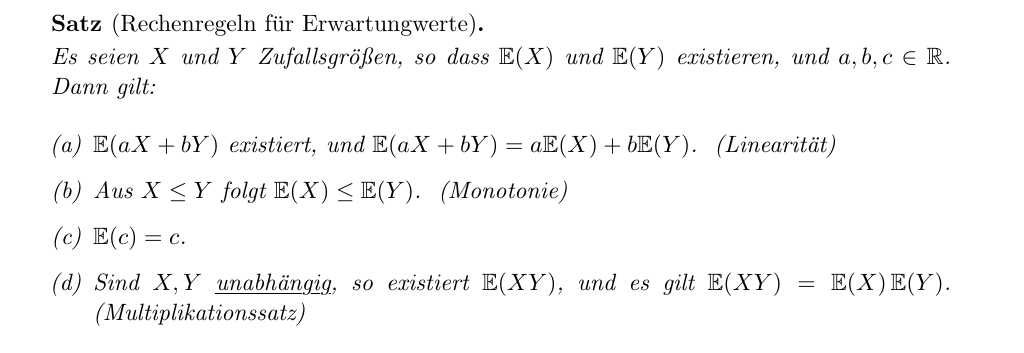
\includegraphics[width=1.0\linewidth]{Rechenregelnerwartungswert}
	\label{fig:rechenregelnerwartungswert}
\end{figure}
\begin{figure}
	\centering
	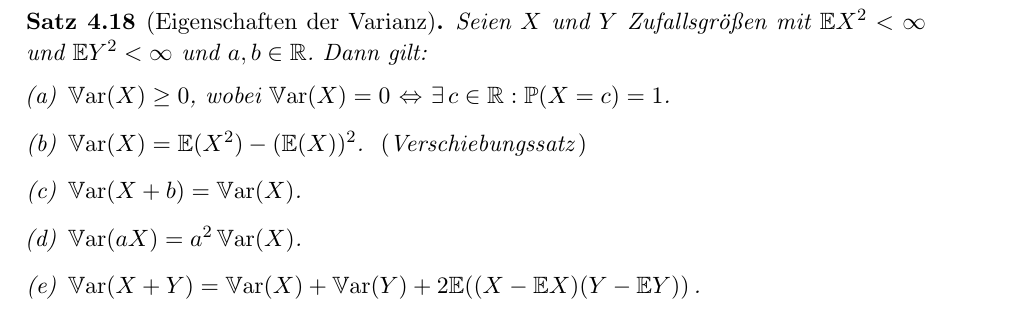
\includegraphics[width=1.0\linewidth]{Rechenregelnvarianz}
	\label{fig:rechenregelnvarianz}
\end{figure}
\begin{figure}
	\centering
	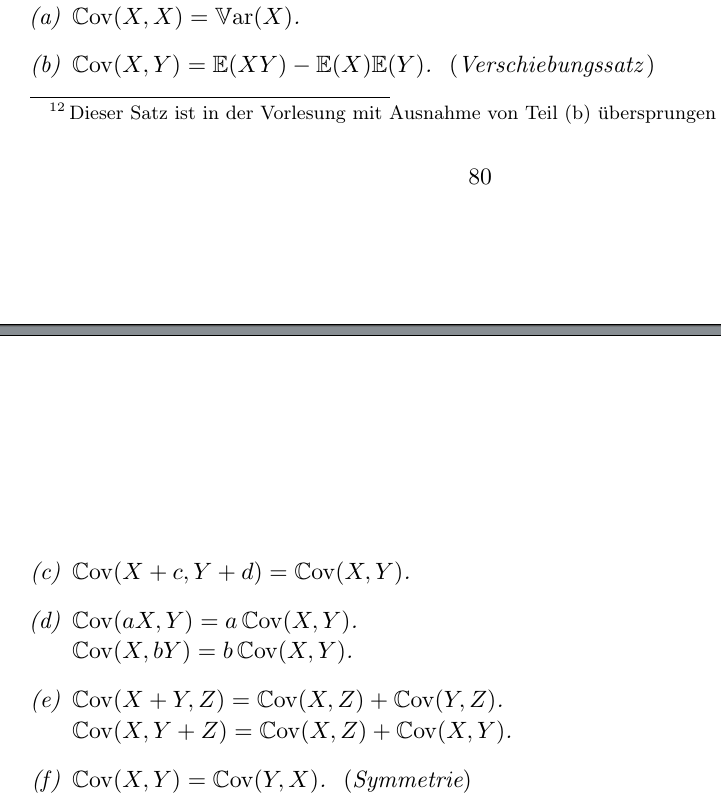
\includegraphics[width=0.5\linewidth]{Rechenregelncovarianz}
	\label{fig:rechenregelncovarianz}
\end{figure}

\newpage
\section{Gesetze der großen Zahlen}
\subsection{schwache}
$\operatorname{P}\left(|R_n - p| \geq \varepsilon \right) \leq \frac{\sigma^2}{\varepsilon^2} = \frac{p(1-p)}{n \varepsilon^2}$  \\
$\rightarrow \forall \epsilon>0 \lim_{n \to \infty} \operatorname{P}\left(|R_n - p| \geq \varepsilon \right) = 0$
\subsection{starke}
$\operatorname{P}\left(\limsup_{n\rightarrow\infty}|\overline{X}_n|=0\right)=1$
\subsection{zentraler Grenzwert}
$\frac{S_n-n\mu}{\sqrt{n \sigma^2}} \underrightarrow{d} Z $
\section{Approximation}
Sei $S_n$ die Summe einer n-stelligen Reihe mit unabhängigen Zufallsgrößen, $\mu$ Erwartungswert, $\sigma^2$ Varianz
normal-aproximierbar mit  (gut bei n über 30) 
$\int_{\frac{a-n\mu}{\sqrt{n\sigma^2}}}^{\frac{b-n\mu}{\sqrt{n\sigma^2}}}$\\
Normalapproximation der Binomialverteilung: $P(a \leq S_n \leq b) \approx \int_{\frac{a-np}{\sqrt{npq}}}^{\frac{b-np}{\sqrt{npq}}} \varphi (x) dx = \phi(\frac{b-np}{\sqrt{npq}}) - \phi(\frac{a-np}{\sqrt{npq}}), q:=1-p $

\section{Statistik}
Produktdichte: $f_\varphi(x):=\prod_{i=1}^{n}\tilde{f}_\varphi(x_i)$\\
Zähldichte:\\
$f_\varphi(x):=$$\binom{n}{k}p^k(1-p)^{n-k}\rightarrow L_k(p)=\binom{n}{k}p^k(1-p)^{n-k}$, k ist Beobachtungswert

Maximum-Likehood-Schätzer: Nimm die größte Likelihoodfunktion \\ 
Likelihood-Funktion: \\ $L_x(\mu)(\vartheta_{ML}(x))=\max_{\vartheta \in \Theta}L_x(\vartheta)$:\\
$f_\mu(x)\rightarrow max$\\
Log-Likelihood: lx($\mu$)=$log L_x(\mu)$, hat dieseelben Maxima und Minima wie die Likehood-funktion

\end{document}
